\section{Evaluating discrete diffusion models using Gradient Moments}
\label{sec:gradient_reference_error}

\begin{figure}[h]
    \centering
    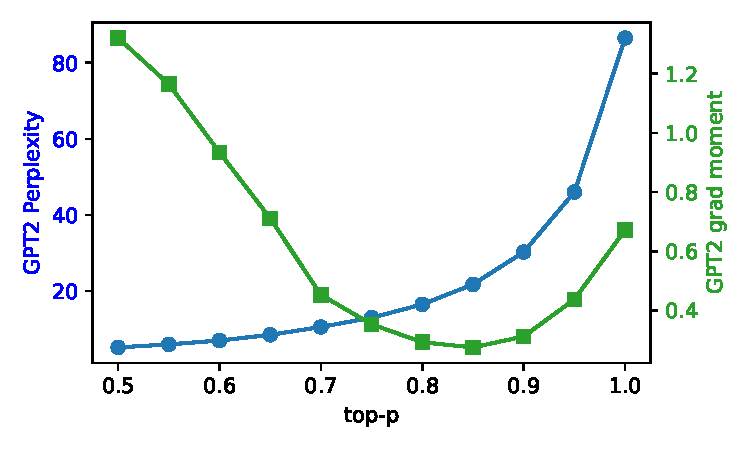
\includegraphics[width=0.6\linewidth]{figures/gpt2_metric.pdf}
    \caption{The perplexity metric keeps improving with lower temperature sampling while the grad moment eventually degrades.}
    \label{fig:gpt2_metric}
\end{figure}

Unlike standard autoregressive language models, distilled discrete diffusion models do not have a tractable sampling likelihood. This means that we cannot evaluate this model class with the standard perplexity metric. For this reason the literature often evaluates these models using \emph{generative perplexity}, where the samples from a discrete diffusion model are processed by an AR model like GPT-2 \citep{radford2019language}, and the perplexity of that AR model on the discrete diffusion samples is reported. The intuition is that samples are judged to be good if a reference LLM assigns a high probability to them. However, this is a flawed premise, as is also discussed in the literature \citep{azzopardi2003investigating,celikyilmaz2020evaluation}: high density samples are often not \emph{typical} \citep{meister2022typical},
meaning that they are not actually similar to the data. An example failure case of the generative perplexity metric is assigning a good score to ungrammatical generated samples that feature many repeated words. Fig.~\ref{fig:gpt2_metric} shows how perplexity and the grad moment metric are affected by top-p sampling. The grad moment eventually degrades when sampling at a low enough temperature.


Here we therefore propose a new metric for evaluating sample quality for discrete diffusion models, the \emph{Gradient Moment} of a reference model. The intuition behind this metric is that while the log-likelihood of a reference AR model on generated samples $\log p_{\theta}^{\text{LLM}}(x)$ is not indicative of sample quality, its \emph{gradient} $\nabla_{\theta} \log p_{\theta}^{\text{LLM}}(x)$ \emph{is}. If an AR model has been trained to convergence on a particular data distribution $q(x)$, its loss gradient on that distribution will be zero: $\mathbb{E}_{q(x)} \nabla_{\theta} \log p_{\theta}^{\text{LLM}}(x) = \mathbf{0}$. Conversely, if the loss-gradient of a trained LLM is large when evaluated on samples $x$, this means that $x$ does not look like the training data. We therefore propose to measure sample quality by the squared norm of this gradient. In practice, our reference LLM may have been trained on a different dataset than the distillation data, or training may not have fully converged: In that case, the loss-gradient evaluated on distillation data is not exactly zero. We therefore correct for this by centering the sample loss-gradient with respect to the data loss-gradient, resulting in the following evaluation metric:
\begin{equation}
\lVert \mathbb{E}_{g}[\nabla_{\theta} \log p_{\theta}^{\text{LLM}}(x)] - \mathbb{E}_{q}[\nabla_{\theta} \log p_{\theta}^{\text{LLM}}(x)] \rVert^2, \label{eq:gpt2moment}
\end{equation}
%\dr{Maybe add a footnote that the expected grad norm on the data is not truly 0 in practice (and on mini-batches), hence the centralization}\tm{+1, seems to make sense, something like, while a maximum likelihood trained model should have $\mathbb{E}_{q} \nabla_{\theta} \approx 0$, in practice this is not strictly the case due to training dynamics (e.g., early stopping) or sampling mini batches of the data.}
where $g$ represents our model's sampling distribution and $q$ is the data distribution. Although this Gradient Moment can be applied to any reference model, in remainder of the paper we choose GPT-2 \citep{radford2019language} as the reference model. The resulting metric is thus the \emph{\ggefull} (\gge). When our sampling distribution is identical to the training data, $g = q$, the metric will attain its lowest possible value of zero. This means that the reference model is unable to distinguish our samples from the ground truth, in the sense that it would not update its parameters when finetuning on our generated data. If the model \emph{is} able to distinguish our samples, the metric will be larger than zero.



In practice we calculate an unbiased stochastic approximation of \eqref{eq:gpt2moment} by calculating gradients on two independent minibatches at a time and taking their inner product.
\begin{equation}
(\nabla_{\theta} \log p_{\theta}^{\text{LLM}}(x^{g}_{1}) - \nabla_{\theta} \log p_{\theta}^{\text{LLM}}(x^{q}_{1}))^{T}(\nabla_{\theta} \log p_{\theta}^{\text{LLM}}(x^{g}_{2}) - \nabla_{\theta} \log p_{\theta}^{\text{LLM}}(x^{q}_{2})), \label{eq:batchgpt2moment}
\end{equation}
where $x^{g}_{1}, x^{g}_{2}$ represent independent batches of samples from our model, and $x^{q}_{1}, x^{q}_{2}$ are independent batches of training data. This stochastic approximation can then be averaged over many batches in order to get a low variance estimate of the quality of our model. This is similar to the loss proposed by \cite{salimans2024multistep} for distilling (continuous) diffusion models, but here we use it as a metric to compare a model to the data distribution, using a reference model as judge.

Although our experiments in this paper are focused on \emph{unconditional generation}, an advantage of the proposed metric is that it is equally valid when conditioning our samples on a prompt or other prefix $x_{c}$: In that case we simply use conditional likelihoods of the form $p_{\theta}^{\text{LLM}}(x|x_{c})$ in the equations above. This is a meaningful advantage of the reference model gradient norm compared to other sampling based methods such as FID \citep{heusel2017gans}.


\section{Experiments}
\label{sec:experiments}
In this section we show that D-MMD can distill discrete diffusion teachers very effectively. Because D-MMD is a stochastic distillation method, we have to rely on metrics that match distributions to study how successful the distillation is. For images we rely on the FID metric, whereas for text we rely on \gge~(see \autoref{sec:gradient_reference_error}).\footnote{The original time of writing of this paper was September 2025.}
\clearpage  % Somehow necessary to get the footnote on this page?

\subsection{CIFAR-10}
\begin{table}[t]
    % \resizebox{\textwidth}{!}{
    \centering
    \begin{tabular}{l|rrrrrrrrr}
        \toprule
         \bfseries Model & 4 & 8 & 16 & 32 & 64 & 128 & 256 & 512 & 1024 \\ \midrule
        Uniform Teacher & & & 36.3 & 17.1 & 10.7 & 8.6 & 7.9 & 7.6 & 7.5 \\
        Uniform D-MMD & 7.1 & 5.0 & 4.1 & \textbf{3.7} & 3.8  \\ \midrule % xid/191308739
        Masked Teacher & & & 122.9 & 47.1 & 20.0 & 11.1 & 7.8 & 6.7 & 6.4 \\
        Masked D-MMD & 22.3 & 12.7 & 5.3 & 3.8 & \textbf{3.5} \\
        \bottomrule
    \end{tabular}
    % }
    \caption{Overview of D-MMD generators and base model sample quality for different NFEs on CIFAR10.
    Results are measured in FID with 50K samples compared to the train dataset. D-MMD models \textit{substantially} outperform their teacher while using a fraction of the NFEs.
    }
    \label{tab:cifar10_overview}
\end{table}

In this first set of experiments we train diffusion models to generate unconditional images.
The models are trained on the 32x32x3 images in the CIFAR10 dataset.
We train a model directly on the $\{0, \ldots, 255\}^{32\times32\times3}$ pixel values, resulting in a total of 3072 tokens that need to be generated.
We evaluate the performance using the FID metric, which notwithstanding the flaws, is still one of the better metrics to measure distances between distributions of (generated) images.

On this dataset we train a masked and uniform diffusion model. These models tend to perform worse than standard diffusion models because there is no inductive bias: every pixel value is a unique token in the vocabulary.
The uniform diffusion teacher achieves an FID of 7.5 and the masked diffusion teacher an FID of 6.4 using 1024 denoising steps.\footnote{Note: continuous (standard) diffusion models easily obtain an FID of around 3 \citep{ho2020denoising}.}


Impressively, D-MMD is able to distill much better generators at only a fraction of the denoising steps compared to the original teacher (\autoref{tab:cifar10_overview}).
For uniform diffusion models an FID of 3.7 is achieved in 32 steps versus an FID of 7.5 for a 1024-step teacher. For Masked diffusion models, the distilled generator outperforms the teacher with 16 steps, and obtains an FID of 3.5 with only 64 uniform denoising steps.
In conclusion, both uniform and masked D-MMD achieve a substantially better Pareto front of steps vs FID than their teachers.

\begin{table}[t]
    % \resizebox{\textwidth}{!}{
    \centering
    \begin{tabular}{l|rrrrrrrrr}
        \toprule
         \bfseries Model & 8 & 16 & 32 & 64 & 128 & 256 & 512 \\\midrule
        % Traditional Uniform Teacher ($p=0.70$) & & & 0.797 & 0.727 & 0.738 & 0.691 & 0.699 & 0.684  \\
        % Traditional Uniform D-MMD ($p=0.70$) & 0.797 & 0.688 & \textbf{0.656} & 0.684 \\ \midrule
        Uniform Teacher ($p=0.50$) & & & 0.375 & 0.326 & 0.330 & 0.324 & 0.313  \\
        Uniform D-MMD ($p=0.70/0.70$) & 0.337 & 0.310 & 0.307 & 0.316 \\ \midrule
        Masked Teacher ($p=0.85$) & & & 0.402 & 0.307 & 0.297 & 0.275 & 0.275 & \\
        Masked D-MMD ($p=0.85$) & 0.456 & 0.236 & \textbf{0.225} & \textbf{0.231} \\ \midrule
        % Masked Teacher (uncentered sqrt) ($p=0.85$) & & & 0.820 & 0.797 & 0.785 & 0.754 & 0.738 & 0.699 \\
        % Masked D-MMD (uncentered sqrt) ($p=0.90$) & 0.824 & 0.731 & 0.691 & \textbf{0.688} \\ \midrule
        AR Baseline & \multicolumn{8}{c}{0.061} \\
        \bottomrule
    \end{tabular}
    % }
    \caption{Text D-MMD generators and base model sample quality for different NFEs measured in \gge~ (see \autoref{sec:gradient_reference_error}).
    %$||\mathbb{E}_{gen}[g_\mathrm{GPT2}(x)] - \mathbb{E}_{data}[g_\mathrm{GPT2}(x)] ||^2$, computed by splitting batches in two and computing the inner product of their gradients.
    D-MMD models outperform their teacher at a fraction of the NFEs.}
    \label{tab:text_mmd_overview}
\end{table}


\subsection{Text}


For text generation we train on Open Web Text (OWT) and take the last $2\%$ as a validation set. Because generative perplexity can be gamed by lower temperature sampling (either intentionally or unintentionally through biased samplers), we use the \gge~ metric to measure distance from the distribution.

Similar to image experiments, we train masked and uniform diffusion teacher models and measure their performance by generating 1024 tokens unconditionally using increasing number of denoising steps. We tune the top-p value for the best \gge. The results are in \autoref{tab:text_mmd_overview}.
The Masked D-MMD generator already outperforms the teacher using only 16 steps, achieving 0.236 \gge.
Similar to the results for images, both the uniform and masked generators consistently outperform their teacher counterparts and improve the whole Pareto front.

\subsection{Block autoregressive diffusion}

\begin{table}[t]
    \centering
    \begin{tabular}{l|rrrrrrrrr}
        \toprule
         \bfseries Model & 16 & 256 \\\midrule
        256-Block Uniform Teacher ($p=0.9$) & - & 0.225  \\
        256-Block Uniform D-MMD ($p=0.7$) & 0.225 & - \\
        \bottomrule
    \end{tabular}
    \caption{Block auto-regressive diffusion model with block size 256. 16-step D-MMD matches the performance of the 256-step teacher.}
    \label{tab:text_mmd_block_ar}
\end{table}



Rather than generating an entire sequence at once, a more realistic setup would be to use a diffusion model to generate a limited block of tokens conditioned on an auto-regressive encoder. This combines the training efficiency and efficient inference of an AR model with the parallel sampling of diffusion. In this experiment, the 16-step D-MMD generator matches the performance of the 256-step teacher (see \autoref{tab:text_mmd_block_ar}).

\begin{table}[t]
    % \resizebox{\textwidth}{!}{
    \centering
    \begin{tabular}{l|rrrrrrrrr}
        \toprule
         \bfseries Method & NFE & FID \\\midrule
         Di4C Teacher & 40 & 8.0 \\
         Di4C (hybrid) & 20 & 9.5 \\
         Di4C & 10 & 20.6 \\
         \midrule
        Uniform Teacher & 512 & 7.6 \\
         & 64 & 10.7 \\
        Uniform D-MMD & 8 & 5.0 \\
        & 16 & 4.1 \\
        & 32 & 3.7 \\ \midrule
        Masked Teacher & 512 & 6.7 \\
         & 64 & 20.0 \\
        Masked D-MMD & 16 & 5.3 & \\
        & 32 & 3.8 & \\
        & 64 & \textbf{3.5} \\
        \bottomrule
    \end{tabular}
    % }
    \caption{Comparison with literature on CIFAR10. D-MMD considerably outperforms existing methods using fewer NFEs.}
    \label{tab:cifar10_related}
\end{table}


\begin{table}[t]
    % \resizebox{\textwidth}{!}{
    \centering
    \begin{tabular}{l|rrrrrrrrr}
        \toprule
         \bfseries Method & NFE & \gge~$\downarrow$ & GPT2 Perplexity $\downarrow$ & Sample entropy \\\midrule
        Duo + DCD & 4 & & 108.2 & 4.82 \\
        Duo + Di4C & 4 & & 150.7 & 4.81 \\
        MDLM + SDTT & 4 & & 339.7 & 5.38 \\
        MDLM + Di4C & 4 & & 239.3 & 5.40 \\
        FMLM & 4 & & 76.4 & 5.05 \\ \midrule
        Masked Teacher  & 256 & 0.275 & 22.5 & 5.13 \\
         & 128 & 0.295 & 23.9 & 5.17 \\
         & 64 & 0.307 & 26.0 & 5.19 \\
        SDTT (reimpl.) & 64 & 0.293 & 26.9 & 5.17 \\
        & 32 & 0.340  & 30.4 & 5.18 \\
        Masked D-MMD
         & 4 & 0.820 & 20.3 & 4.60\\
         & 16 & 0.236 & \textbf{17.2} & 5.00 \\
        & 32 & \textbf{0.225} & 19.4 & 5.05 \\ \midrule
        Data & & 0.000 & 15.4 & 5.44 \\ \midrule
        \textcolor{gray}{Masked Teacher} & \textcolor{gray}{256} & \textcolor{gray}{0.672} & \textcolor{gray}{85.9} & \textcolor{gray}{5.59} \\
        \textcolor{gray}{($p=1.0$)} & \textcolor{gray}{128} & \textcolor{gray}{0.711} & \textcolor{gray}{91.1} & \textcolor{gray}{5.61} \\
        & \textcolor{gray}{64} & \textcolor{gray}{0.781} & \textcolor{gray}{101.0} & \textcolor{gray}{5.63} \\
        \textcolor{gray}{Masked D-MMD} & \textcolor{gray}{4} & \textcolor{gray}{0.719} & \textcolor{gray}{66.1} & \textcolor{gray}{5.44} \\
        \textcolor{gray}{($p=1.0$)} & \textcolor{gray}{16} & \textcolor{gray}{0.558} & \textcolor{gray}{67.7} & \textcolor{gray}{5.57} \\
        & \textcolor{gray}{32} & \textcolor{gray}{0.578} & \textcolor{gray}{72.1} & \textcolor{gray}{5.57} \\
        \bottomrule

    \end{tabular}
    % }
    \caption{Comparison with literature on OWT measured in \gge~(lower is better), generative perplexity (should not be too high) and sample entropy (should not be too low). D-MMD is able to achieve even better results in fewer steps.}
    \label{tab:text_related}
\end{table}

\begin{table}[t]
    % \resizebox{\textwidth}{!}{
    \centering
    \begin{tabular}{ll|rrrrrrrrr}
        \toprule
         \bfseries D-MMD Masked & & 4 & 8 & 16 & 32 & 64 \\ \midrule
        without noise & (FID) & 151\textcolor{white}{.0} & 37.0 & 14.7 & 7.7 & 6.0 \\
        \hspace{.5cm} & (generator output entropy) & 1.26 & 1.37 & 1.57 & 1.86 & 1.91 \\ \midrule
        with noise & (FID) & 22.3 & 12.7 & 5.3 & 3.8 & \textbf{3.5} \\
        \hspace{.5cm} &(generator output entropy) & 1.01 & 1.29 & 1.53 & 1.76 & 1.83 \\
        \bottomrule
    \end{tabular}
    % }
    \caption{Noise input conditioning is important for masked distillation. Fewer steps require more generator output collapse, and generators with noise conditioning can collapse their factorized output distribution more.
    }
    \label{tab:cifar10_noiseinput}
\end{table}


\subsection{Comparison related work}
In this section we compare to the discrete diffusion distillation literature. For Di4C, results in the main paper are available on CIFAR10. Note that Di4C is actually at an advantage here, because its teacher model is trained using a discrete process that mimics the destruction of a Gaussian process. As a result, Di4C is able to achieve a teacher FID of 8.0 using only 40 steps. Nevertheless, because D-MMD outperforms the teacher models it still outperforms Di4C with 5.0 using only 8 steps with the uniform generator (see \autoref{tab:cifar10_related}).

Recall that a metric such as generative perplexity is roughly measuring your distance from a mode, and collapsed models can easily score generative perplexities near 1.0\footnote{For example the sentence "hahahahahahaha" repeated also has a perplexity near 1.0} (the optimum). Instead, we measure performance with \ggefull~(\gge), which is somewhat more robust to this. Here we do see that even though SDTT improves upon the teacher model, it still degrades over repeated distillation rounds and is outperformed by D-MMD (see \autoref{tab:text_related}). Especially the \gge~metric highlights this degradation. The optimal top-p was chosen at $p=0.85$ by sweeping, measuring \gge~on the masked teacher. SDTT (reimpl.) and D-MMD use the same teacher. For completeness, we also show results without top-p $p = 1.0$. For other related works, \citep{sahoo2025diffusion,roos2026categorical} the results were taken from \citep{lee2026one}.


\subsection{Conditioning the generator on input noise}
In theory the generator should have access to a noise source to be able to generate a distribution. However, in \citet{salimans2024multistep} it was noted that in practice no input noise is required for Gaussian diffusion distillation. However, in the case of 1-step masked generation \citep{zhu2025dimo} noise conditioning turned out to be important. For images we learn a projection of a 2D Gaussian noise pyramid to be added to the residual. For text we learn a projection of plain Gaussian noise.

In our case we find that masked distillation performs much better with an extra noise source (see \autoref{tab:cifar10_noiseinput}). In that case, the generator is able to collapse its output distribution more and achieves much better sample quality. In contrast, for uniform diffusion we did not observe any meaningful improvements. As is the case with Gaussian diffusion, for uniform diffusion there may already be sufficient noise in $z_t$ that the generator is able to use. All other masked distillation experiments in this paper condition on input noise.

\subsection{Discussion on students outperforming teachers}
It may seem counterintuitive that students can outperform their teachers. However, teachers are trained using maximum likelihood which is known to be mode-covering. Mode-collapsing behavior is often induced by reducing temperature or top-p sampling.

Many distillation approaches such as D-MMD have an adversarial component and generate samples based on the student, which both are reminiscent of reverse-KL optimization. D-MMD may move more density towards modes without fully collapsing, which is typically desired for samples from an image or language generator.

A paradoxical side-effect is the following: suppose the student is better than the teacher for a certain number of steps. Then, the student's performance will degrade at some point even as sampling steps increase, as that performance will converge to the teacher's at high step counts.
